% Why SA generates novel sequences but only recalls faces.
% Faces (top): the convex blend IS the output -> blur -> recall.
% Proteins (bottom): a per-position arg max quantizes the blend -> recombinant.
% Real data. Compile: pdflatex Fig_blend_decode.tex
\documentclass[border=12pt]{standalone}
\usepackage{graphicx}
\usepackage{tikz}
\usepackage{amsmath}
\usepackage[T1]{fontenc}
\usetikzlibrary{positioning,arrows.meta,calc}

\definecolor{rec}{RGB}{0,120,150}       % recombined site (family-legal, != nearest)
\definecolor{seqdark}{RGB}{45,45,45}
\definecolor{seqgray}{RGB}{170,170,170}
\definecolor{good}{RGB}{36,130,70}
\definecolor{bad}{RGB}{190,55,55}
\definecolor{rule}{RGB}{210,210,210}
\definecolor{sub}{RGB}{110,110,110}

% generated seq #4 vs nearest natural #42 (real); recombined sites (differ from
% nearest, but family-legal) in teal, the rest dark; reference row in gray.
\newcommand{\genseqrow}{\textcolor{seqdark}{L}\,\textcolor{seqdark}{F}\,\textcolor{rec}{\textbf{V}}\,\textcolor{seqdark}{G}\,\textcolor{rec}{\textbf{N}}\,\textcolor{seqdark}{L}\,\textcolor{rec}{\textbf{P}}\,\textcolor{seqdark}{P}\,\textcolor{rec}{\textbf{D}}\,\textcolor{seqdark}{T}\,\textcolor{seqdark}{T}\,\textcolor{seqdark}{E}\,\textcolor{seqdark}{E}\,\textcolor{rec}{\textbf{E}}\,\textcolor{seqdark}{L}\,\textcolor{seqdark}{K}\,\textcolor{rec}{\textbf{E}}\,\textcolor{seqdark}{F}\,\textcolor{rec}{\textbf{F}}\,\textcolor{rec}{\textbf{S}}\,\textcolor{seqdark}{Q}\,\textcolor{rec}{\textbf{F}}\,\textcolor{seqdark}{G}\,\textcolor{rec}{\textbf{P}}\,\textcolor{seqdark}{V}\,\textcolor{seqdark}{V}\,\textcolor{rec}{\textbf{S}}\,\textcolor{seqdark}{V}}
\newcommand{\refseqrow}{\textcolor{seqgray}{L}\,\textcolor{seqgray}{F}\,\textcolor{seqgray}{I}\,\textcolor{seqgray}{G}\,\textcolor{seqgray}{G}\,\textcolor{seqgray}{L}\,\textcolor{seqgray}{A}\,\textcolor{seqgray}{P}\,\textcolor{seqgray}{Y}\,\textcolor{seqgray}{T}\,\textcolor{seqgray}{T}\,\textcolor{seqgray}{E}\,\textcolor{seqgray}{E}\,\textcolor{seqgray}{N}\,\textcolor{seqgray}{L}\,\textcolor{seqgray}{K}\,\textcolor{seqgray}{L}\,\textcolor{seqgray}{F}\,\textcolor{seqgray}{Y}\,\textcolor{seqgray}{G}\,\textcolor{seqgray}{Q}\,\textcolor{seqgray}{W}\,\textcolor{seqgray}{G}\,\textcolor{seqgray}{K}\,\textcolor{seqgray}{V}\,\textcolor{seqgray}{V}\,\textcolor{seqgray}{D}\,\textcolor{seqgray}{V}}

\newcommand{\badge}[2]{\tikz[baseline]{\node[rounded corners=3pt,fill=#1,text=white,font=\sffamily\bfseries\small,inner xsep=8pt,inner ysep=3pt,anchor=base]{#2};}}

\begin{document}
\begin{tikzpicture}[font=\sffamily,>=Stealth,
  hdr/.style={font=\sffamily\bfseries\large,anchor=west},
  sub/.style={font=\sffamily\small\itshape,text=sub,anchor=west},
  rlab/.style={font=\sffamily\footnotesize\itshape,text=sub,anchor=east},
  seq/.style={font=\ttfamily\large,anchor=west},
  stat/.style={font=\sffamily\small,text=black!75,anchor=west},
  flab/.style={font=\sffamily\footnotesize,text=sub,anchor=north},
  arr/.style={->,line width=1pt,sub}]

% ===================== BAND 1: FACES (top) =====================
\node[hdr] (fh) at (0,0) {Olivetti face};
\node[sub] at ($(fh.east)+(0.25,0)$) {pixels: the convex blend \emph{is} the output\,---\,you see a blur};

\node[anchor=north west] (fA) at (0.4,-0.6) {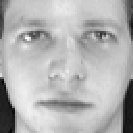
\includegraphics[width=1.8cm]{bd_faceA.pdf}};
\node[anchor=west,font=\Large] (pl) at ($(fA.east)+(0.3,0)$) {$+$};
\node[anchor=west] (fB) at ($(pl.east)+(0.3,0)$) {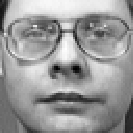
\includegraphics[width=1.8cm]{bd_faceB.pdf}};
\draw[arr] ($(fB.east)+(0.25,0)$) -- node[above,font=\sffamily\footnotesize\itshape,text=sub]{blend} ($(fB.east)+(1.9,0)$);
\node[anchor=west] (fbl) at ($(fB.east)+(2.1,0)$) {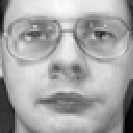
\includegraphics[width=1.8cm]{bd_faceBlend.pdf}};
\node[flab] at (fA.south) {stored A};
\node[flab] at (fB.south) {stored B};
\node[flab,text=bad] at (fbl.south) {blurry ghost};

\node[stat,text width=5.6cm,align=left] (fc) at ($(fbl.east)+(0.55,0.55)$)
  {No quantizer: the blend itself is the image\,---\,not a valid new face. So the clean output is a \textbf{verbatim stored image} (\textbf{cosine 1.00}).};
\node[anchor=north west] at ($(fc.south west)+(0,-0.12)$) {\badge{bad}{RECALL}};

% ===================== divider =====================
\draw[rule,line width=1pt] (0,-3.5) -- (16.4,-3.5);

% ===================== BAND 2: PROTEINS (bottom) =====================
\node[hdr] (ph) at (0,-4.0) {Protein sequence};
\node[sub] at ($(ph.east)+(0.25,0)$) {a per-position \texttt{arg\,max} \emph{quantizes} the blend\,---\,you get a recombinant};

\node[rlab] (gl) at (2.8,-5.05) {SA-generated};
\node[seq,right=4pt of gl] (gr) {\genseqrow};
\node[rlab] (nl) at (2.8,-5.6) {nearest natural};
\node[seq,right=4pt of nl] (nr) {\refseqrow};
\node[stat,anchor=west,font=\sffamily\footnotesize\itshape,text=sub] at ($(nr.south west)+(0,-0.35)$)
  {\textcolor{rec}{\textbf{teal}} = sites recombined away from the nearest natural (each is still a residue the family uses there)};

\node[stat] (ps) at (0,-6.85)
  {every residue is one the family uses at that site (\textbf{71/71}, \textcolor{good}{valid}) \;\;$\bullet$\;\; \textbf{38\%} of sites recombined ($62\%$ identity to nearest, \textcolor{good}{novel}) \;\;$\bullet$\;\; passes RRM \textbf{HMM}};
\node[stat] (ps2) at (0,-7.4)
  {The convex blend lives in embedding space; \texttt{arg\,max} snaps each of the 71 sites to one residue, so the \emph{average is never seen}\,---\,different sites inherit from different neighbors.};
\node[anchor=north west] at ($(ps2.south west)+(0,-0.18)$) {\badge{good}{NOVEL + VALID}};

\end{tikzpicture}
\end{document}
